%!TEX root = ../../../main.tex
\section[Coupling \Nds to Optical Antennas]{Coupling \Nds to Double Bowtie Antenna Structures} \label{sec::coupling_antennas}

	Plasmonic nanoantennas are very recent devices designed to efficently convert freely propagating optical radiation into localized energy and vice versa \cite{Optical Antennas, Palash Bharadwaj, Bradley Deutsch, and Lukas Novotny, nancy::77, nancy::78}. Leveraging this unique property, integrating \sivs with optical antennas creates coupled systems with a range of desireable features. These include enhanced \pl emission and the ability to tailor \pl spectra of the integrated emitters. The latter can be achieved by tuning the physical design parameters of the system including antenna geometry and emitter placement.

	In this chapter we report on our efforts aimed at enhancing the properties of \sivs by coupling them to optical double bowtie antennas. To this end we transfer selected \nds containing \sivs to the target antenna structure using \pp methods. After successful coupling we investigate the integrated structure experimentally. In addition to that we successfully relate some of our results to theoretical predictions.

	In the following we give a short discussion of the most important properties of optical antennas. Then we sketch the actual coupling process and report on the optical properties of the resulting integrated structure.

	\subsection{Plasmonic Antennas}

		Optical nanoantennas act as convertes between propagating and localized electro-magnetic fields. Thus, they can be used efficiently to couple photons in and out of nanoscale objects \cite{Curto2010}. Due to their small physical sizes, comarale or smaller than the \wl of visible light, they are capable of focusing optical fields to subdiffraction-limited volumes, offering the ability to manipulate electromagnetic fields at nanoscales \cite{Curto2010::3, nancy::78}. This property, dubbed sub-wavelength confinement, has successfully been exploited to enahnce the excitation and emission of quantum emitters \cite{Curto2010::4, Curto2010::5, Curto2010::6, Curto2010::7} and to modify their spectra \cite{Curto2010::8}. Resulting practical applications include near-field optical microscopy \cite{nancy::79}, surface enhanced spectroscopy \cite{nancy::80, nancy::81} and molecular sensing \cite{nancy::82}.

		A nanoantenna is a nanostructure made from materials such as noble metals like gold or silver. These metals have in common that they are very susceptible to being polarized by electro-magnetic fields. When illuminated by the incident electromagnetic radiation causes electrons in the metal to behave as a plasma that tends to move with respect to the atomic lattice. As a result excess charge at the opposite surfaces of the material accumulates and the material becomes temporarily polarized until restoring forces equillibrate the charge distribution.

		Thus incident light of a given frequency induces oscillations in the free electron gas density in the surface layers of the metal. At resonance these light-induced oscillations exhibit modes of standing waves. The quasi-particles associated with these modes are known as \lsps (\LSPs).
		For an in-depth treatment of \LSPs in the context of nanoantennas we refer the reader to \cite{nancy::thesis} and references therein.

		Here it suffices to say, that \LSPs facilitate the deciding property of optical antennas: Converting electromagnetic energy from the far-field into localized energy in the near-field. This allows, in combination with the high collection-efficencies of nanoantennas, to efficiently couple visible radiation with wavelenghts of hundres of nanometers, into small effective spatial volumes of only a few nanometer in diameter.

		To create a controlled hot-spot several antenna designs are possible. In the context of this thesis we rely on double bowtie antennas available via a collaboration with \nancy. \autoref{fig::double_bowtie_antenna_schematic} illustrates the typical bowtie antenna.

		\begin{figure}[thp]
				\centering
				\testbox{\includegraphics[trim = 0 0 0 0,  clip= true, width = 0.5\textwidth]{./pics/double_bowtie_antenna_schematic.png}}
				\caption[Schematic of a double bowtie antenna]{Schematic of a double bowtie antenna \cite{nancy::thesis, Rahbany2015, Rahbany2016}.}
				\label{fig::double_bowtie_antenna_schematic}
		\end{figure}

		This antenna design utilizing a symmetric arrangement of four identical triangle-shaped blocks, separated by a small gap. This setup allows \LSP modes local to individual blocks to couple with each other resulting in the formation of an intense hot-spot in the center area \cite{nancy::85}, see \autoref{fig:double_bow_tie_hotspot}. The actual electromagnetic response of a double bowtie nanoantenna depends on its physical design parameters such as gap size, material used, geometry and size. Furthermore, properties of incident light such as \wl and polarization determine antenna operation.

		\begin{figure}[thp]
				\centering
				\testbox{\includegraphics[trim = 0 0 0 0,  clip= true, width = 0.5\textwidth]{./pics/antenna_fdtd_simulation_field.png}}
				\label{fig::double_bow_tie_hotspot}
				\caption[Hot-spot of a double bowtie antenna]{Simulation result of the electric field map of a gold double bowtie nanoantenna \cite{nancy::thesis, Rahbany2015, Rahbany2016}. The structure has gap of $d = \SI{150}{nm}$, a side length of $L = \SI{2}{\micro\meter}$ and a thickness of $S = \SI{60}{nm}$. The center of the antenna exibits an area of pronouced focus, the so-called hot-spot.}
		\end{figure}


		The improved electromagnetic field at the center of a metallic nanoantenna can be used to increase the spontaneous emission rate of emitters emitting at frequencies close to the resonance frequency of the antenna. This result is the known as Purcell effect \cite{nancy::86}. The gap between the antenna arms acts as a resonant cavity providing a strong near field interaction with the emitter. This interaction modiefies the density of states of the system, effectively providing additional modes for the emitter to decay into, thus amplifying its total decay rate. The amplification affects both radiative and non-radiative decay.
		The magnitude of the amplification for an emitter is quantified by the ratio of its enhanced decay rate to its free space decay rate, known as the Purcell factor $F_p$. This factor is proportional to $Q/V_{eff}$ where $Q$ denotes the quality of the antenna and $V_{eff}$ the volume of the hot-spot. Thus antenna desing must optimize $F_p$ as a necessary condition for significant enhancement of \fl emission.

		In addition to the antennas local field enhancment, the emitters original quantum yield $\eta_0$ influences the overall effectiveness of the emission enhancement. From theoretical considerations \cite{nancy::thesis, nancy::140, nancy::162, nancy::163}, the modified quantum efficiency $\eta$ of the combined system consisting of emitter and antenna can be obtained as

		\begin{equation}
			\eta = \frac{\eta_0}{\frac{1-\eta_0}{F_p} + \frac{\eta_0}{\eta_{ant}} },
		\end{equation}

		where $\eta_{ant}$ denotes the fraction of \fl which is not dissipated through losses in the metal of the antenna. It is clear that an emitter with $\eta_0 \to 1$ will not profit from the Purcell effect. On the contrary, for realisitc antennas with $\eta_{ant} < 1$ antenna-induced losses reduce the overall quantum yield $\eta$. Consequently poor emitters with low initial $\eta_{0}$ stand to profit the most from antenna-emitter coupling provided antennas are engineered well, \i.e.\ they maximize their Purcell Factors and minimize their losses. For an in-dept review

		The presented considerations illustrate that due to their relatively low quantum efficiency, \sivs are excellent candidates for coupling with antennas. Thus it is promising to expliot the improved electromagnetic field at the center of a double bowtie antenna to enhance the spontaneous emission rate of \sivs and thus improve their merit as \spss.

	\subsection{Plasmonic Antenna Design and Simulation} \label{sec::structure_antenna}

		 To couple \sivs to optical antennas, we work with gold double bowtie antennas on a gold substrate. In comparison with triangular, or single bowtie antennas, double bowtie antennas offer significantly improved intensity enhancements. Antennas were provided by \nancy in a joined effort to explore the possibilities of combining antennas with \sivs. The antennas themselves were fabricated using electron beam lithography, a technique suitable to imprint predetirmined patterns onto a suitable substrate with nanoscale resolution \cite{nancy::232}. \autoref{subfig::antenna_structures_sem} shows a SEM image of an array of antenna structures of various sizes. In \autoref{subfig::antenna_one_structure_sem} a detail of an individual double bowtie antenna is shown. It can be seen that the double bowtie antenna is placed in the center of another structure, a so-called bulls-eye antenna, consisting of multiple concentric gratings. When illuintated by a laser at a proper angle, the gratings excite surface plasmon polaritons (SPPs) which are directed towards the center of the structure. If a double bowtie antenna is present in the center, SPPs can interact with the \LSPs of the double bow tie, leading to an even stronger localization of electromagnetic fields in the gap of the bowtie. While this interaction certainly merits exploration in the context of enhancing \sivs, we omit the excitation of SSPs in our first exploration of the couling of \sivs and antennas. Thus the presence of the gratings can be ignored for our purposes. The reader interested in the details of bulls-eye antennas and their properties is referred to \cite{nancy::thesis}.

		 		\begin{figure}[htp]
		 			\begin{subfigure}[t]{ 0.49\linewidth}
		 				\centering
		 				\testbox{\includegraphics[trim = 0 0 0 0,  clip= true, width = 0.7\textwidth]{./pics/Antenna2_upper_right_150923_01.png}}
		 				\caption{}
		 				\label{subfig::antenna_structures_sem}
		 			\end{subfigure}
		 			\hfill
		 			\begin{subfigure}[t]{ 0.49\linewidth}
		 				\centering
		 				\testbox{\includegraphics[trim = 0 0 0 0,  clip= true, width = 0.7\textwidth]{./pics/Ir27M_mitte_213_151111_13.jpg}}
		 				\caption{}
		 				\label{subfig::antenna_one_structure_sem}
		 			\end{subfigure}
		 			\caption[SEM images of double bowtie structures.]{SEM images of antenna structures. (a) Overview of a field of antenna structures exhibiting various dimensions. (b) Detail of one antenna sturcture. In the middle the double bowtie design is visible. A grating structure consisting of multiple gratings is surrounding it.}
		 		\end{figure}

		To effectively enhance the emission of an emitter by coupling it to an optical antenna, the emission \wl must match the resonant \wl of the antenna. In the context of \sivs a value of \SI{738}{nm} is required. Since this value can be considered constant, the design parameters of the antenna must be choose such, that the resulting resonance matches it. An additional constraint is placed on the size of the antenna gap, since it must be big enough to accomodate \nds hosting \sivs, the former are around \SI{100}{\nm} in size. However, it cannot be choosen arbitrarily big, since bigger gaps lead to larger effectiv volumes and thus smaller Purcell Factors.

		Using finite time difference domain (FDTD) simulaton deploying Lumerical Software the design space of gold double bowtie nanoantennas on a gold substrate was explored \cite{nancy::thesis}. Although we initially attempted to simulate antennas without a \nd present in the gap, it was subsequently discovered that its ab initio inclusion yielded superior results. Thus to determine usable design parameters for our purposes, an integrated system combining antenna and \nd was used. To better mimick experimental conditions and associated imprefections, the \nd was placed slightly off-center in the gap.

		In a series of simulation it was established that a gapsize of $d = \SI{150}{nm}$, a side length of $L = \SI{2}{\micro\meter}$ and a structure thickness of $S = \SI{60}{nm}$ are feasible parameters as refered to in \autoref{double_bowtie_antenna_schematic}. The simulation required the index of refraction for gold which was taken from Palik \cite{Palik, E. D. Handbook of optical constants of solids. 3, (Academic press, 1998)}.

		The resulting geometry hosting a \nd is capable of producing a suitable hotspot when excited.

		\begin{figure}[htp]
				\centering
				\testbox{\includegraphics[trim = 0 0 0 0,  clip= true, width = 0.5\textwidth]{./pics/antenna_fdtd_simulation_spectrum.png}}
			\caption[Simulation of the resonance spectrum of a double bowtie antenna]{FDTD simulation of the electric field intensity of a double bowtie nanoantenna as as a function of the \wl of incident light. Two peaks are identified. The major peak corresponds exceptionally well with \siv emission at \SI{738}{nm}. The minor peak is attributed to the presence of a \nd.}
			\label{fig::antenna_fdtd_spectrum}
		\end{figure}

		Finally, to pin-point the resonant \wl for the antenna hosting a \nd, the electric field intensity is simulated as a function of the \wl of the incident light. The resulting spectrum is shown in \autoref{fig::antenna_fdtd_spectrum}. Two resonant peaks are found. The intense major peak at \SI{739}{nm} coincides exceptionally well with the \siv emission wavelength \SI{738}{nm} indicating successful antenna design. In addition to the major peak, an additional minor mode at a lower wavelength of \SI{710}{nm} is found \cite{Rahbany2016}. We remark that if the \nd in the gap of the antenna is removed from the simulations, the minor feature vanishes. Thus the additional peak is well-attributed to the presence of the \nd.

		In summary, the combined simulation results suggest, that the engineered system of nanoantenna and \nd is well suited to effectively enhance the emission from an \siv hosted in the \nd. In the following sections we report on the experimental realization of this preposition.

	\subsection{\siv in a Plasmonic Double Bowtie Antenna}
		%
		% \begin{figure}[htp]
		% 	\centering
		% 	\testbox{\includegraphics[trim = 0 0 0 0,  clip= true, width = 0.3\textwidth]{./pics/ccd_s1_g3_db_g150_d20_rightone_crop.png}}
		% 	\caption{CCD image recorded in the confocal setup of an antenna structure under white light illumination. In the middle, the \nd containing multiple \sivs had been placed.}
		% 	\label{fig::place_ccd}
		% \end{figure}

		In the following we report on our attempts to couple \sivs to double bowtie antennas. Given ideal \nds containing exactly one \siv each, the major challenge of coupling consists of transporting a given \nd to the gap of an antenna. However, \nds rarely contain exactly one \siv. The identification of a perfect candidate requires manual examination of hundreds of \nds, making it an extremely tedious, error-prone and time-consuming process. In addition to that, methods such as \pp entail a very real risk of permanently damaging or invalidating a precious candidate in transit to the antenna, thus rendering the significant efforts invested in identifying the candidate futile. In contrast to that, \nds containing anything from a small number to an entire ensemble of \sivs are much more likely and thus easier to identify and to use.

		Thus we approach the problem of coupling \sivs to antennas in several phases. In the first phase \nds containing an entire ensemble of \sivs are utilized. Such \nds can be found with high probability. Due to the large number of individual emitters involved, they exhibit an increased resilence against being damaged. The disadvantage is that once placed in the antenna, the whole ensemble will be affected by Purcell enhancement and as a result its effectiveness for individual emitters cannot be obtained.

		After gaining experience in the first phase, the second phase aims at using \nds with a very low number of \sivs hosted. Here the goal is to identify a candidate \nd in a reasonable amount of time. Once transferred to an antenna using \pp methods, saturation and second order correlation measurements can be attempted provided the involved emitters remain stable.

		The third and last phase focuses on identifying a \nd hosting a singleton \siv building onto of the insights gained in the previous phases. After successful \pp transit, a precise characterization of the emitter and its antenna-induced Purcell enhancement should be possible.

		Here we report on our obtained results regarding phases one and two. At the time of writing this, phase three was not yet implemented.

\section[Antennas]{Coupling \Nds to Double Bowtie Antenna Structures} \label{sec::coupling_antennas}

	In this chapter, the integration of \sivs in nanodiamonds with double bowtie nanoantenna structures is presented.
	The emission from the coupled system has two advantages:
	\begin{itemize}
		\item The antenna causes an enhancement in the \siv{}'s \pl emission intensity.
		\item The \pl spectrum of the nanodiamond is modified depending on the geometry of the nanoantenna as well as the position of the emitter in the gap. This provides the flexibility of designing the nanoantennas to accurately predict and tune the emitters' PL spectrum as desired.
	\end{itemize}

	% \begin{figure}[tp]
	% 	\begin{subfigure}[t]{ 0.49\linewidth}
	% 		\centering
	% 		\testbox{\includegraphics[trim = 0 0 0 0,  clip= true, width = \textwidth]{./pics/Ir27M_mitte_213_151111_18.jpg}}
	% 		\caption{}
	% 		\label{subfig::nd_before_pick_hr}
	% 	\end{subfigure}
	% 	\hfill
	% 	\begin{subfigure}[t]{ 0.49\linewidth}
	% 		\centering
	% 		\testbox{\includegraphics[trim = 0 0 0 0,  clip= true, width = \textwidth]{./pics/Ir27M_mitte_213_151111_21.png}}
	% 		\caption{}
	% 		\label{subfig::nd_before_pick_no_hr}
	% 	\end{subfigure}
	% 	\caption{caption}
	% \end{figure}

	\begin{figure}[tp]
		\begin{subfigure}[t]{ 0.49\linewidth}
			\centering
			\testbox{\includegraphics[trim = 0 0 0 0,  clip= true, width = \textwidth]{./pics/pick_colored.png}}
			\caption{}
			\label{subfig::pick_antenna_sem}
		\end{subfigure}
		\hfill
		\begin{subfigure}[t]{ 0.49\linewidth}
			\centering
			\testbox{\includegraphics[trim = 0 0 0 0,  clip= true, width = \textwidth]{./pics/Ir27M_mitte_213_151111_26_colored.png}}
			\caption{}
			\label{subfig::transfer_antenna_sem}
		\end{subfigure}
		\caption{Pick and Place technique for nanodiamond manipulation, nanodiamond colored blue in the image for better visibility. (a) A \nd sticking to the nanomanipulator tip which was lifted off the substrate (b) Transfer of the \nd to the target antenna structure which is in the background.}
	\end{figure}


	\begin{figure}[tp]
		\centering
		\testbox{\includegraphics[trim = 0 0 0 0,  clip= true, width = 0.5\textwidth]{./pics/place_colored.png}}
		\caption{SEM detail image of the middle of the double bowtie antenna structure with the transferred \nd. Vor better visibility, the \nd is colored blue. Antenna damage caused by the placement of the \nd is visible as black area at the tip of the top triangle}
		\label{fig::place_antenna_sem}
	\end{figure}

	\subsection{Plasmonic Antennas}

		nancy Doktorarbeit:
		Plasmons can be considered as a collective oscillation of the free electron density on the surface of a conducting material.
		\\
		Localized surface plasmons (LSP) are the result of stationary resonant oscillations of the surface charge density at the boundaries of metallic nanostructures [37,38]. Due to their significant optical properties, LSPs are shown to enhance electromagnetic field confinement.
		\\
		Plasmonic nanoantennas have proven to be very successful candidates in tailor- ing light propagation and confinement at the nanoscale. Electromagnetic antennas are defined as metallic devices used for receiving and transmitting electromagnetic waves. In addition to acting as probing devices, antennas must also serve as direc- tional devices that optimize and accentuate radiation energy in some directions and suppress it in others [77]. Optical nanoantennas benefit from their sizes, which are comparable to or smaller than the wavelength of visible light, to overcome the diffraction limit and manipulate electromagnetic fields at the nanoscale [78]. This allows them to be widely used in many applications such as near-field op- tical microscopy [79], surface enhanced spectroscopy [80,81], sensing [82], medical therapy [83], and optoelectronic devices [84].
		When light is incident on metallic nanoantennas, modes of standing waves are created at resonance. This creates an electric field enhancement in their vicinity. A good nanoantenna is characterized by its high collection efficiency (large cross sec- tion), and its ability to focus incident electromagnetic light into sub-wavelength ar- eas (large near-field enhancement). To improve their performance, researchers have found that cutting a gap in the center of nanoantennas leads to a higher near-field enhancement while maintaining the same effective cross-section [85]. This occurs due to the coupling between the LSP modes of the two parts of the nanoantenna creating a hotspot in the gap.
		Exciting LSPs can be simply achieved by res- onantly illuminating nanostructures with electromagnetic waves.
		\\
		\cite{Curto2010}
		Optical antennas, acting as converters between propagating and localized fields,provide an effective route to couple photons in and out of nanoscale objects. These antennas are the counterparts of conventional radio and microwave antennas and operate in the visible regime (1, 2). Optical antennas have been shown to focus optical fields to subdiffraction- limited volumes (3), enhance the excitation and emission of quantum emitters (4–7), and modify their spectra (8).
		\\
		A characteristic of antennas is their directed emission and reception. So far, the control of directionality has mainly been pursued by photonic crystal structures (9) and surface-plasmon–based devices (10–12). However, for such structures approaching the nanometer scale diffraction can limit the collimated beaming of light. On the other hand, the interaction of quantum emitters with light is best enhanced with microcavities(13, 14). Compared with these approaches, plasmonic nanoantennas offer a much smaller footprint in an open geometry combining strong subwavelength fields and increased transitionrates, together with the prospect of directionality.
		\\
		\cite{Giessen2010}
		from gold, a metal that can develop charge oscillations in its surface layers when excited by optical radiation. These antennas allow visible radia- tion, which has wavelengths of hundreds of nanometers, to couple into a semiconductor quantum dot only a few nanometers in diam- eter, and also direct the emission
		\\
		Good mode- matched antennas reradiate their energy after excitation within a single cycle of the wave. Molecules or quantum dots take nanoseconds or even longer to reradiate their energy. This time scale corresponds to about 1 million oscillations at optical frequencies, and the emission is in all directions.
		\\
		If an atom, molecule, or quantum dot is placed into the near-field of a metallic nanoantenna (within about 1/50th the wavelength of the emitted radiation), its excited state can radiate photons very efficiently to free space (see the fi g- ure, panel B). The quantum emitters can emit a single photon, which can be exploited in quantum optics. Additionally, the nanoantenna can redirect radiation into a defined solid angle in space and impose a specifi c polarization on it.
		\\
		The demonstration of the Purcell effect, which is the acceleration of the decay of the quantum emitter caused by impedance matching by the antenna to free space, could also enhance the radiative emission over nonradiative losses
		\\
		\cite{Novotny2011}
		The electro- magnetic antenna, originally referred to as an ‘aerial’, is a transducer between electromagnetic waves and electric currents, and generally operates in the radiofrequency regime. In analogy with the electro- magnetic antenna, we define the optical antenna as a device thatconverts freely propagating optical radiation into localized energy, and vice versa1.The spatial extent of a receiver or transducer is commonly much smaller than the wavelength of radiation, λ, and is typically of the order of λ/100.
		\\
		Surface plasmon resonances make optical antennas particularly efficient at selected frequencies. A generic antenna problem is illustrated in Fig. 3. It consists of a transmitter and a receiver, both represented by dipoles p. The antenna is introduced to enhance the transmission efficiency from the transmitter to the receiver. This enhancement can be achieved by increasing the total amount of radiation released by the trans- mitter, for which the antenna efficiency is a useful figure of merit:
		\begin{equation}
			p=p
		\end{equation}
		where P is the total power dissipated by the antenna, Prad is the radiated power and Ploss is the power dissipated through other means,such as by absorption in the antenna. However, the transmission efficiency can also be improved by directing the radiation in the direction of the receiver. The efficiency for this process is repre- sented by the directivity:
		\begin{equation}
			p=p
		\end{equation}
		where the angles θ and ϕ represent the direction of observation and p(θ,ϕ) is the angular power density. The combination of antenna effi- ciency and directivity is referred to as the antenna gain:
		\begin{equation}
			p=p
		\end{equation}
		By reciprocity, we can interchange the fields and sources in Fig. 3 to give p1• E2 = p2 • E1, where E1 (E2 ) is the field of dipole p1 (p2 ) evalu- ated at the location of p2 (p1). A good transmitting antenna is therefore also a good receiving antenna. For a transmitter in the form of a two-state quantum emitter, reciprocity leads to a relationship between the emitter’s excitation rate Γexc and its spontaneous emission rate:
		\begin{equation}
			p=p
		\end{equation}
		Here, the superscript ‘o’ refers to the absence of the antenna and the subscript ‘θ’ indicates the polarization state; that is, the electric field vector points in direction of the θ unit vector. An equivalent equation holds for polarization in the ϕ direction. Interestingly, exci- tation in a direction of high directivity allows the excitation rate to be enhanced more strongly than the radiative rate. Another important antenna parameter is the antenna aperture, which is formally the same as the absorption cross-section sigma. Let us consider a dipole-like receiver with a cross-section σo that is not cou- pled to an antenna. The unit vector in the direction of the absorption dipole axis is denoted as np and the incident field at the location of the receiver is Eo . Once we couple the receiver to an antenna, the field at the receiver increases to E and the cross-section or antenna aperture becomes1
		\begin{equation}
			p=p
		\end{equation}
		Thus, the aperture of an optical antenna scales with the local intensity enhancement factor. Theoretical and experimental stud- ies have shown that intensity enhancements of 104–106are readily achievable14,36,37 and hence, for typical molecules with ‘free-space’ cross-sections of sigmao = 1 nm2 , we find that a layer of molecules spaced 0.1–1 μm apart can absorb all of the incident radiation if each molecule is coupled to an optical antenna. Of course, this estimate ignores the coupling between antennas and therefore has limited validity.

	\subsection{Plasmonic Antenna Design} \label{sec::structure_antenna}

		\begin{figure}[tp]
			\begin{subfigure}[t]{ 0.49\linewidth}
				\centering
				\testbox{\includegraphics[trim = 0 0 0 0,  clip= true, width = \textwidth]{./pics/Antenna2_upper_right_150923_01.png}}
				\caption{}
				\label{subfig::antenna_structures_sem}
			\end{subfigure}
			\hfill
			\begin{subfigure}[t]{ 0.49\linewidth}
				\centering
				\testbox{\includegraphics[trim = 0 0 0 0,  clip= true, width = \textwidth]{./pics/Ir27M_mitte_213_151111_13.jpg}}
				\caption{}
				\label{subfig::antenna_one_structure_sem}
			\end{subfigure}
			\caption{SEM images of the antenna structures. (a) Overview of a field of antenna structures exhibiting various dimensions. (b) Detail of one antenna sturcture. In the middle the double bowtie design is visible. The ring grating structure is surrounding it.}
		\end{figure}

		\begin{figure}[tp]
			\centering
			\testbox{\includegraphics[trim = 0 0 0 0,  clip= true, width = 0.3\textwidth]{./pics/ccd_s1_g3_db_g150_d20_rightone_crop.png}}
			\caption{CCD image recorded in the confocal setup of an antenna structure under white light illumination. In the middle, the \nd containing multiple \sivs had been placed.}
			\label{fig::place_ccd}
		\end{figure}

		\begin{figure}[tp]
			\centering
			\testbox{\includegraphics[trim = 0 0 0 0,  clip= true, width = 0.5\textwidth]{./pics/antenna_fdtd_simulation_spectrum.png}}
			\caption{FDTD calculations of the electric field intensity as a function of wavelength in the gap of a double bowtie nanoantenna containing a nanodiamond.}
			\label{fig::antenna_fdtd_calculation}
		\end{figure}

		FDTD numerical simulations were performed using Lumerical software to characterize gold double bowtie nanoantennas on a gold substrate. The nanoantennas are tailored to have a gap of g = \SI{150}{nm} (taking into account the diameter of the nanodiamonds of around \SI{100}{nm}), side length of L = \SI{2}{\micro\meter}, and a thickness of t = \SI{60}{nm} (see Fig.3a).
		Upon excitation with incident light, an intense electromagnetic hotspot is formed in the nanoantenna gap \cite{Rahbany2015}\todo{read paper}, which is expected to excite a nanodiamond containing SIV centers aiming to enhance its fluorescence emission.
		Unlike a single bowtie that is sensitive only to the polarization along its principle axis (C2 rotational symmetry), a double bowtie features a C4 rotational symmetry and therefore focuses both parallel and perpendicular polarizations (i.e. all in-plane directions).
		% For that, a circularly polarized light with a wavelength range of λ = 400 - 1500 nm is chosen to illuminate a gold double bowtie nanoantenna on a gold substrate, which efficiently excites both the horizontal and vertical components of the structure.
		The index of refraction of gold is taken from Palik \cite{}\todo{Palik, E. D. Handbook of optical constants of solids. 3, (Academic press, 1998)}, and that of the nanodiamond is chosen to be n = 2.4 at $\lambda$ = \SI{660}{nm}.
		The electric field intensity in the nanoantenna gap is then measured as a function of wavelength to identify the antenna resonance.
		The spectrum is given in \cref{fig::antenna_fdtd_calculation} where we observe that the resonance shows two peaks; an intense peak coinciding with the SiV emission wavelength ($\lambda$ = \SI{739}{nm}), and an additional mode at a lower wavelength ($\lambda$ = \SI{710}{nm}) \cite{Rahbany2016}
		The resonance spectrum of the antenna alone shows only one peak at \SI{739}{nm}.
		Thus, the additional peak is attributed to the presence of the nanodiamond that is slightly shifted from the center of the gap, corresponding to our experimental conditions.
		These calculations suggest, that the emission from an \siv at \SI{738}{nm} is effectively enhanced and directed by the antenna.
		\\
		High optical confinement can be reached via successful SPP-LSP coupling at the nanoscale. One way of achieving that is by integrating diffraction gratings with nanoscale apertures or nanoantennas. Nanoantennas have shown to be very good candidates for focusing and enhancing electromagnetic fields in their vicinity. Nevertheless, due to their small size, a significant amount of the incident light is lost either by being scattered, reflected, or not entirely focused on the nanoantenna. On the other hand, plasmonic gratings act as sources for launching and orienting SPPs in a specific desired direction. Integrating a nanoantenna in the center of a concentric plasmonic ring grating creates a highly focused electromagnetic field at its center leading to an increase in the radiative decay rate as well as a collimated radiation of a dipole emitter placed inside [nancy::238–240]
		aus Nancys Doktorabreit al ERlaerung, warum die antenne ringe herum hat
		\todo{fehlt Erklaerung zu Ringen}
		Optical plasmonic focusing has been extensively studied in the field of nanoplasmon- ics and has very important applications in high resolution imaging, sensing, waveg- uiding, nanolithography, and sub-wavelength optics. For this purpose, researchers have investigated several plasmonic structures capable of enhancing and confining surface plasmons into sub-wavelength dimensions. Cavities composed of diffraction gratings acting as SPP launchers can be used as efficient nanoscale focusing de- vices [243,244], confined surface plasmon polariton amplifiers [245], and fluorescence emission enhancement tools [246] (Fig. 4.1a). It has been shown that the plasmonic “Bull’s Eye” structure, made of periodic concentric grooves in a metallic substrate, can lead to a strongly enhanced evanescent field focused in its center where propa- gating surface plasmons constructively interfere [247]. Controlling the directionality of transmitted light through an aperture surrounded by periodic corrugations was also achieved, which allows overcoming the limitations of low transmittance and high diffraction in the sub-wavelength regime [248]. In a similar study, the aperture is replaced by a narrow slit in the center of the Bull’s Eye antenna leading to a higher power coupling, narrower radiated beam, and good return losses [249]. In addition, ring grating structures can be used to control the luminescence directivity of emitters placed in the center. Fluorescence beaming of molecules placed in a nanoaperture surrounded by concentric metallic grooves was studied by directing their emission in a precise direction and with a specific angular width depending on their wavelength [250]. Similar work related to the fluorescence emission of quan- tum dots placed in a slit surrounded by a ring grating shows that their emission can be manipulated to form perfectly narrow collimated beams [251] (Fig. 4.1b). Ring gratings surrounding diamond nanoposts [186] and circular diamond nanowires [135] with embedded nitrogen-vacancy (NV) centers were also used to improve the collec- tion efficiency and radiative decay rate of single NV centers. Directing the far-field emission of single NV centers placed in the center of a Bull’s Eye grating was also recently investigated in a study that resulted in a high collection efficiency within a low numerical aperture [252]. This motivates us to use the ring grating structure described below to study efficient plasmon-emitter coupling at the nanoscale. An interesting property of the device is that the position of excitation determines the direction of propagation of the SPPs, providing a flexible mean of studying their interactions with molecules or dipole-like emitters placed on the surface.

	\subsection{\sivs in a Plasmonic Double Bowtie Antenna}

		\begin{figure}[htp]
			\centering
			\testbox{\includegraphics[trim = 0 0 0 0,  clip= true, width = 0.3\textwidth]{./pics/ccd_s1_g3_db_g150_d20_rightone_crop.png}}
			\caption{CCD image recorded in the confocal setup of an antenna structure under white light illumination. In the middle, the \nd containing multiple \sivs had been placed.}
			\label{fig::place_ccd}
		\end{figure}

			% Einleitung
			In the following, we discuss specific details and challenges concerning our initial attempts of coupling \sivs to plasmonic double bowtie nanoantennas. Furthermore, we assert successful coupling and report spectroscopic measurements of an \siv situated inside the gap of the antenna.
			\\
			% additional methods
			When transferring \nds to the center of an antenna, we distinguish between \nds hosting
			To transfer individual \nds hosting one or more \sivs to the center of an antenna, we follow two approaches:
			First we chose a \nd containing several \sivs for \pp and afterwards a \nd containing a single \siv.
			As mentioned before, single \sivs may be damaged by the electron radiation in the SEM during \pp and stop emittig \pl light.
			Hence, we decided to run first experiments with \nds containing multiple \sivs.
			This approach has the advantages that we are able to gain experience in the execution of the \pp process without the risk of permanently damaging the emitter and therefore rendering the tedious \pp process futile.
			For measurements of the intensity enhancement by the antenna, a single emitter is necessary.
			However, the antenna's influence on the \siv spectrum can be studied when serveral emitters are present.
			Therefore, studies of the spectrum are performed in this first approach.
			\\
			% Spectroscopic measurements
			After this deterministic placement, the antenna sample is placed in the confocal setup.
			The structure where the \nd was placed is searched observing the sample surface in a CCD image under white light illumination (\cref{fig::place_ccd}).
			A scan of the antenna is performed in the confocal setup using the \SI{660}{nm} \cw laser of the setup.
			The scan serves to locate the middle of the antenna structure and therefore the \nd which had been placed there.
			An outline of the rings is visible in an overview scan of the antenna structure (\cref{subfig::antenna_laser_scan}).
			Zooming in to the middle of these rings, some of the edges of the bowtie antenna are vaguely visible (\cref{subfig::antenna_bowtie_laser_scan}).
			This images suffices to approach the \nd close enough to measure a PL spectrum.
			The PL spectrum of the \siv in the nanodiamond gives insight to the effect of the nanoantenna on its emission.
			The result is displayed in \cref{subfig::spectrum_antenna_nd_multiple}.
			To rule out artifacts, a spectrum of an antenna of the same dimensions without \nd is recorded (\cref{subfig::spectrum_antenna_no_nd}).
			% Fig. 7a where an increase in the PL intensity is observed by more than a factor 10 indicating that the nanoantennas indeed contribute to the enhancement of the SiV centers emission.
			% A $\lambda$ = 710 nm long pass filter is used to eliminate any signal from the laser.
			The additional peak at a lower wavelength is attributed to the antenna resonance mode.
			To verify this, we convolute the experimental PL spectrum of the nanodiamond measured before placing it in the nanoantenna (\cref{subfig::spectrum_nd_multiple}) with the intensity spectrum of the nanoantenna obtained by simulations (\cref{fig::antenna_fdtd_calculation}).
			The resulting spectrum is given in \cref{subfig::antenna_convolution}, and is in good agreement with the measured spectrum in \cref{subfig::spectrum_antenna_nd_multiple}, confirming that indeed the extra peak is due to the antenna resonance.


			\begin{figure}[tp]
				\begin{subfigure}[t]{ 0.49\linewidth}
					\centering
					\testbox{\includegraphics[trim = 0 0 0 0,  clip= true, width = \textwidth]{./pics/spe_Ir27M_f200_xy04x13y88_D09_t30_highP_fit.pdf}}
					\label{subfig::spectrum_nd_multiple}
					\caption{}
				\end{subfigure}
				\hfill
				\begin{subfigure}[t]{ 0.49\linewidth}
					\centering
					\testbox{\includegraphics[trim = 0 0 0 0,  clip= true, width = \textwidth]{./pics/antenna_no_ND.pdf}}
					\caption{}
					\label{subfig::spectrum_antenna_no_nd}
				\end{subfigure}
				\caption{(a) PL spectrum of the emitter in the preselected nanodiamond at room temperature. Black: experimental results; red: fit to experimental data, \todo[inline]{verfnuenftige fehlergrenzen einfuegen}which yields a \ZPL \cwl of \SI{738.55\pm0.01}{nm} and a \lw of  \SI{5.09\pm0.03}{nm}}
			\end{figure}

			\begin{figure}[tp]
				\begin{subfigure}[t]{ 0.49\linewidth}
					\centering
					\testbox{\includegraphics[trim = 0 0 0 0,  clip= true, width = \textwidth]{./pics/xy_scan-11_2APD.png}}
					\caption{}
					\label{subfig::antenna_laser_scan}
				\end{subfigure}
				\hfill
				\begin{subfigure}[t]{ 0.49\linewidth}
					\centering
					\testbox{\includegraphics[trim = 0 0 0 0,  clip= true, width = \textwidth]{./pics/xy_scan-13_2APD.png}}
					\caption{}
					\label{subfig::antenna_bowtie_laser_scan}
				\end{subfigure}
				\caption{(a) Confocal scan of the double bowtie antenna where a \nd containing multiple \sivs had been placed. The rings are visible. (b) Detail scan of the triangles of the same antenna structure, which make up the double bowtie antenna. While the seperate triangle cannot be seen, some edges and two bright spots are visible. To identify the place of the \nd we compare the middle point of the rings in (a), the point of intersection of the edges and the bright spot and conclude that the upper bright spot in (b) is the location of the \nd. }
			\end{figure}

			% \begin{figure}[tp]
			% 	\centering
			% 	\testbox{\includegraphics[trim = 0 0 0 0,  clip= true, width = 0.3\textwidth]{./pics/antenna_no_ND.pdf}}
			% 	\caption{<caption>}
			% 	\label{fig::spectrum_antenna_multiple_before}
			% \end{figure}

			\begin{figure}[tp]
				\begin{subfigure}[t]{ 0.49\linewidth}
					\centering
					\testbox{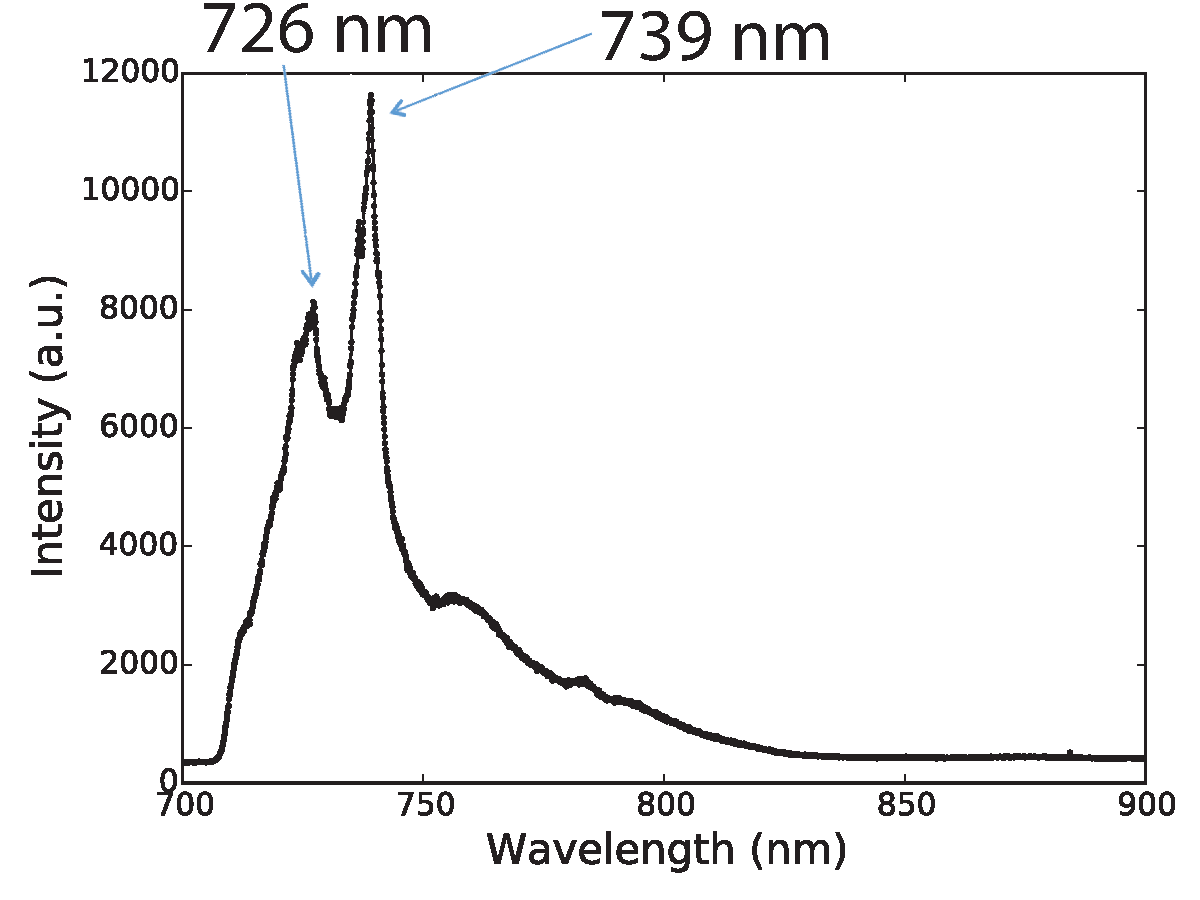
\includegraphics[trim = 0 0 0 0,  clip= true, width = \textwidth]{./pics/find_middle_with_ccd_highP_2_arrows.pdf}}
					\caption{}
					\label{subfig::spectrum_antenna_nd_multiple}
				\end{subfigure}
				\hfill
				\begin{subfigure}[t]{ 0.49\linewidth}
					\centering
					\testbox{\includegraphics[trim = 0 0 0 0,  clip= true, width = \textwidth]{./pics/antenna_convolution.png}}
					\caption{}
					\label{subfig::antenna_convolution}
				\end{subfigure}
				\caption{(a) Measured PL spectrum of the emitter after placing the \nd into the nanoantenna, (b) Convolution of the spectrum of the measured PL spectrum of the emitter before \pp (see Figure \ref{subfig::spectrum_nd_multiple}) and the simulated resonance spectrum of the nanoantenna (see Figure \ref{fig::antenna_fdtd_calculation}).}
			\end{figure}

		\subsubsection{\Nd With Few \siv Coupled to Antenna}\label{subsubsection::antenna_single_siv}

			As the experiment of coupling a \nd with an ensemble of \sivs proved to be very successful, the next step was to select a \nd with only few \sivs, i.e. that it exhibits countrate saturation and a dip in the \gtf.
			In this section, coupling a \nd containing only few \sivs to a double bowtie antenna is reported.
			It is an intermediate step between coupling
			% sample description
			The origin sample used for this experiment is an \ir substrate onto which a solution of \nds were drop-casted.
			Starting material for the \nds was a electronic grade diamond film produced by the company rho-BeSt coating (now CarbonCompetence)\todo{checken, ob angaben passen}.
			It was then milled in a \basd process\footnote{\krueger} to \nds of a size of \todo{groesse einfuegen}.
			The \nds were drop-casted at \SI{60}{\celsius} onto an \ir substrate containing cross markers which had been treated with Piranha etch.
			% sample M02-16: drop-casted with SiGH45
			\\
			% preselection,
			Preselecting a \nd with a single \siv is imposes additional constrains to the suitability of an \nd if compared to a \nd with multiple \sivs.
			First, only a small percentage of the technically suited \nds (size, isolation) contain a single \siv, second, damage due to electon radiation during \pp.
			% position
			The position of the \sivs on the substrate surface was performed in the same way as described in \cref{subsubsection::
			}.
			The identification whether bright spots in the scan were suitable emitter was performed as follows:
			First a saturation curve was recorded.
			Countrate saturation is only a necessary and not a sufficient measure for single photon emission, hence the saturation measurement alone does not prove that the emitter in question is single.
			However, it takes only a few seconds to record a saturation measurement compared to potentially hour-long measurements of \gtfs.
			Therefore, it is a quick selection method to evaluate potential candidates.
			Once an emitter with a saturating countrate was found, a spectrum was recorded to prove that the emitter in question is indeed an \siv.
			At last, the \gtf was recorded.
			We successfully found an \siv with a small dip in the \gt function.
			While the dip is too small to account for a single \siv, it indicates the presence of only few \sivs.
			% transfer
			Hence, we proceeded by transferring the host \nd to the antenna structure.
			\\
			% Spectroscopic measurements
			The \siv coupled to the antenna structure was then spectroscopically investigated in the confocal setup.
			First, we recorded a spectrum (spectrum A).
			The result of the first recorded spectrum revealed a multitude of peaks.
			To ensure that the peaks are no artifacts due to deficient alignment, we rechecked the alignment which proved to be precise.
			We initiated another measurement of the spectrum.
			However, this time the recorded spectrum only showed a broad \bkg (spectrum B).
			After checking in the confocal scan that the measurement was performed at the correct position, we had to conclude that the emitter bleached shortly after recording spectrum A.
			\\
			As mentioned earlier, the electron radiation may damage \sivs in nanodiamonds.
			The electron radiation might have put the \siv into an unstable state.
			Although we were still able to measure one spectrum, further application of energy from the laser seems to have permanently bleached the \siv.
			While we cannot solidify this conclusion with further experimental evidence, we observed in earlier independent measurements that some \sivs bleach after electron radiation and that some \sivs bleach after an extended laser irradiation \cite{}.
			The observations in this measurement suggest a combination of the two effects.
			\\
			We performed FDTD calculations of the selected \siv in the host \nd in the plasmonic double bowtie antenna as described in the previous section\todo{put in pictures}.
			We used spectrum B to for \bkg correction of spectrum A and fitted the measured peaks (\cref{subfig::single_siv_spec_after_transfer_antenna_bkg_corrected}).
			In the simulations, we do not see the peaks between \SIrange{700}{750}{nm} that we recorded in the measurement.
			Hence, we conclude, that not additionally to the observed photobleaching, also the emitter's spectrum was modified in the \pp process.
			While it is not possible to pinpoint exactly which circumstance caused the modification, possible candidates are\todo{enter candidates and explain why}.
			\\
			To gain further insight, we performed FDTD calculations with antenna damage and different dipole orientation.
			To be able to include the dipole orientation into the calculations, a dipole emitter with a broad emission instead of a narrow emission peak has to be used.
			Therefore, the convolution method as described in the previsous section is more adequate for our purpose, as the \siv exhibits a very narrow emission peak.
			However, these calculations give further insight.
			First, the antenna damage does not have a big effect on the spectra, however the dipole orientation changes the results drastically (\cref{}).
			Therefore, future experiments should include polarization measurements to experimentally quantify the impact of the emitter orientation.

			\begin{figure}[tp]
				\begin{subfigure}[t]{ 0.49\linewidth}
					\centering
					\testbox{\includegraphics[trim = 0 0 0 0,  clip= true, width = \textwidth]{./pics/g2_sat113_5mW_corr_fit.pdf}}
					\caption{}
					\label{subfig::single_siv_g2_before_transfer_antenna}
				\end{subfigure}
				\hfill
				\begin{subfigure}[t]{ 0.49\linewidth}
					\centering
					\testbox{\includegraphics[trim = 0 0 0 0,  clip= true, width = \textwidth]{./pics/sat114_fit_bkg.pdf}}
					\caption{}
					\label{subfig::single_siv_sat_before_transfer_antenna}
				\end{subfigure}
				\caption{(a) The \gtf of the preselected \nd hosting few nanodiamonds. A dip at \gtz is present, however it does not decrease below 0.5. While this indicates that more than one \siv is present, a small number of \sivs cause a dip in the \gtf instead of no dip at all which would be measured under coherent emission\todo[inline]{cps zu a.u. aendern}. (b) Saturation curve of the same emitter\todo[inline]{zahlen fuer sat eintragen}. Data points are black, fitted curve red.}
			\end{figure}

			\begin{figure}[tp]
				\begin{subfigure}[t]{ 0.49\linewidth}
					\centering
					\testbox{\includegraphics[trim = 0 0 0 0,  clip= true, width = \textwidth]{./pics/single_spectrum_sat113_fit.pdf}}
					\caption{}
					\label{subfig::single_siv_spec_before_transfer_antenna}
				\end{subfigure}
				\hfill
				\begin{subfigure}[t]{ 0.49\linewidth}
					\centering
					\testbox{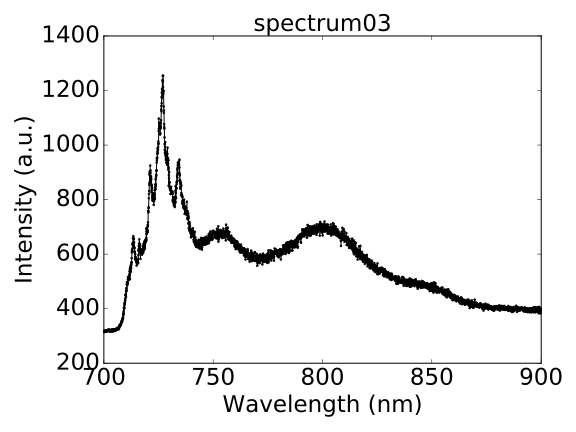
\includegraphics[trim = 0 0 0 0,  clip= true, width = \textwidth]{./pics/spectrum03.pdf}}
					\caption{}
					\label{subfig::single_siv_spec_after_transfer_antenna}
				\end{subfigure}
				\caption{(a) Spectrum of the preselected \nd hosting few \sivs. (b) Measured spectrum after transfer of the preselected \nd into the double bowtie antenna.}
			\end{figure}

			% \begin{figure}[tp]
			% 	\centering
			% 	\testbox{\includegraphics[trim = 0 0 0 0,  clip= true, width = 0.5\textwidth]{./pics/single_spectrum_sat113_fit.pdf}}
			% 	\caption{<caption>}
			% 	\label{fig::single_siv_spec_before_transfer_antenna}
			% \end{figure}

			\begin{figure}[tp]
				\begin{subfigure}[t]{ 0.49\linewidth}
					\centering
					\testbox{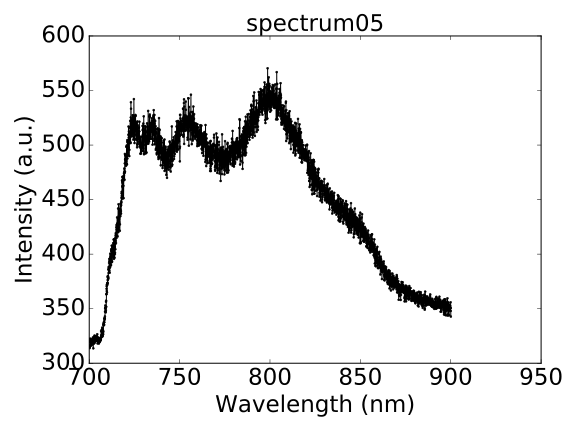
\includegraphics[trim = 0 0 0 0,  clip= true, width = \textwidth]{./pics/spectrum05.pdf}}
					\caption{}
					\label{subfig::single_siv_spec_bkg_antenna}
				\end{subfigure}
				\hfill
				\begin{subfigure}[t]{ 0.49\linewidth}
					\centering
					\testbox{\includegraphics[trim = 0 0 0 0,  clip= true, width = \textwidth]{./pics/spectrum_sat113_fit_origin.pdf}}
					\caption{}
					\label{subfig::single_siv_spec_after_transfer_antenna_bkg_corrected}
				\end{subfigure}
				\caption{(a) Spectrum of the \nd hosting few \sivs coupled to the double bowtie antenna after the emitter bleached. (b) Background corrected spectrum of the transferred \nd in the double bowtie antenna. Peaks are fitted, results of the fits are the colored lines. For background correction, the spectrum in (a) was used.}
			\end{figure}

		\subsubsection{Outlook: Coupling a \Nd With a Single \Siv to the Plasmonic Double Bowtie Antenna}
			To effectivly state the emission enhancement of the \siv by the plasmonic double bowtie antenna, a single \siv is necessary.
			A correct measure for the emission enhancement is the saturation count rate.
			The saturation countrate is proportional to the inverse of the emitter's lifetime.
			Hence, if there are two or more emitters present, photons of the individual emitters are emitted randomly, which renders a correct saturation measurement impossible.
			However, finding \sivs in \nds which fulfill both spectroscopic (\gtz $\approx$0, saturation, narrow \ZPL spectrum) and technical (size, isolation of \nds) constraints tured out to be a very time-consuming work.
			\\
			We investigated different kinds of \nds in the search of \nds exhibiting optimal spectroscopic and technical parameters.
			We were able to fulfill the size requirements posed by the \pp process and antenna design by producing different patches of different sizes of \nds and took the ones which were best suited.
			We also developped a good isolation of the \nds on the substrate by treating the \ir substrate with Piranha etch and tuning the amount of diamond solution drop-casted onto the substrate.
			This leaves us with the need of a higher propability of exactly one \siv per \nd.
			Parameters which have an impact on the quantity of \sivs per \nd are the initial \siv density in the starting material and the \nd size.
			Once the time constraint of finding a single \siv in a \nd is overcome, we can apply the extensive methods and knowledge gained by the reported procedures to couple a single \siv to a plasmonic bowtie antenna.
			\\
			To our knowledge, our experiments were the first time an \siv in a \nd was coupled to a plasmonic bowtie antenna.
			The extraordinarily precise correlation of the theoretically predicted and the experimentally recorded spectrum of an ensemble of \sivs in a \nd make this process a promising candidate for future applications.
